\documentclass[12pt]{extreport}
\usepackage[T2A]{fontenc}
\usepackage[utf8]{inputenc}        % Кодировка входного документа;
                                    % при необходимости, вместо cp1251
                                    % можно указать cp866 (Alt-кодировка
                                    % DOS) или koi8-r.

\usepackage[english,russian]{babel} % Включение русификации, русских и
                                    % английских стилей и переносов
%%\usepackage{a4}
%%\usepackage{moreverb}
\usepackage{amsmath,amsfonts,amsthm,amssymb,amsbsy,amstext,amscd,amsxtra,multicol}
\usepackage{indentfirst}
\usepackage{verbatim}
\usepackage{tikz} %Рисование автоматов
\usetikzlibrary{automata,positioning}
\usepackage{multicol} %Несколько колонок
\usepackage{graphicx}
\usepackage[colorlinks,urlcolor=blue]{hyperref}
\usepackage[stable]{footmisc}

\usepackage[linesnumbered]{algorithm2e}   
\usepackage{MnSymbol,wasysym}

\usepackage{graphicx}
\usepackage{listings}
\graphicspath{ {.} }

%% \voffset-5mm
%% \def\baselinestretch{1.44}
\renewcommand{\theequation}{\arabic{equation}}
\def\hm#1{#1\nobreak\discretionary{}{\hbox{$#1$}}{}}
\newtheorem{Lemma}{Лемма}
\theoremstyle{definiton}
\newtheorem{Remark}{Замечание}
%%\newtheorem{Def}{Определение}
\newtheorem{Claim}{Утверждение}
\newtheorem{Cor}{Следствие}
\newtheorem{Theorem}{Теорема}
\theoremstyle{definition}
\newtheorem{Example}{Пример}
\newtheorem*{known}{Теорема}
\def\proofname{Доказательство}
\theoremstyle{definition}
\newtheorem{Def}{Определение}



\DeclareMathOperator{\Cov}{Cov}
\DeclareMathOperator{\Var}{Var}
\DeclareMathOperator{\Corr}{Corr}
\DeclareMathOperator{\E}{\mathop{E}}
\DeclareMathOperator{\Med}{Med}
\DeclareMathOperator{\Mod}{Mod}
\DeclareMathOperator*{\plim}{plim}

%% \newenvironment{Example} % имя окружения
%% {\par\noindent{\bf Пример.}} % команды для \begin
%% {\hfill$\scriptstyle\qed$} % команды для \end


% одеваем шапки на частые штуки
\def \hb{\hat{\beta}}
\def \hs{\hat{s}}
\def \hy{\hat{y}}
\def \hY{\hat{Y}}
\def \he{\hat{\varepsilon}}
\def \hVar{\widehat{\Var}}
\def \hCorr{\widehat{\Corr}}
\def \hCov{\widehat{\Cov}}

% Греческие буквы
\def \a{\alpha}
\def \b{\beta}
\def \t{\tau}
\def \dt{\delta}
\def \e{\varepsilon}
\def \ga{\gamma}
\def \kp{\varkappa}
\def \la{\lambda}
\def \sg{\sigma}
\def \tt{\theta}
\def \Dt{\Delta}
\def \La{\Lambda}
\def \Sg{\Sigma}
\def \Tt{\Theta}
\def \Om{\Omega}
\def \om{\omega}

% Готика
\def \mA{\mathcal{A}}
\def \mB{\mathcal{B}}
\def \mC{\mathcal{C}}
\def \mE{\mathcal{E}}
\def \mF{\mathcal{F}}
\def \mH{\mathcal{H}}
\def \mL{\mathcal{L}}
\def \mN{\mathcal{N}}
\def \mU{\mathcal{U}}
\def \mV{\mathcal{V}}
\def \mW{\mathcal{W}}

% Жирные буквы
\def \mbb{\mathbb}
\def \RR{\mbb R}
\def \NN{\mbb N}
\def \ZZ{\mbb Z}
\def \PP{\mbb{P}}
\def \QQ{\mbb Q}



%\date{22 июня 2011 г.}
\let\leq\leqslant
\let\geq\geqslant
\def\MT{\mathrm{MT}}
%Обозначения ``ажуром''
\def\BB{\mathbb B}
\def\CC{\mathbb C}
\def\RR{\mathbb R}
\def\SS{\mathbb S}
\def\ZZ{\mathbb Z}
\def\NN{\mathbb N}
\def\FF{\mathbb F}
%греческие буквы
\let\epsilon\varepsilon
\let\es\varnothing
\let\eps\varepsilon
\let\al\alpha
\let\sg\sigma
\let\ga\gamma
\let\ph\varphi
\let\om\omega
\let\ld\lambda
\let\Ld\Lambda
\let\vk\varkappa
\let\Om\Omega
\def\abstractname{}

\def\R{{\cal R}}
\def\A{{\cal A}}
\def\B{{\cal B}}
\def\C{{\cal C}}
\def\D{{\cal D}}

%классы сложности
\def\REG{{\mathsf{REG}}}
\def\CFL{{\mathsf{CFL}}}


%%%%%%%%%%%%%%%%%%%%%%%%%%%%%%% Problems macros  %%%%%%%%%%%%%%%%%%%%%%%%%%%%%%%


%%%%%%%%%%%%%%%%%%%%%%%% Enumerations %%%%%%%%%%%%%%%%%%%%%%%%

\newcommand{\Rnum}[1]{\expandafter{\romannumeral #1\relax}}
\newcommand{\RNum}[1]{\uppercase\expandafter{\romannumeral #1\relax}}

%%%%%%%%%%%%%%%%%%%%% EOF Enumerations %%%%%%%%%%%%%%%%%%%%%

\usepackage{xparse}
\usepackage{ifthen}
\usepackage{bm} %%% bf in math mode
\usepackage{color}
%\usepackage[usenames,dvipsnames]{xcolor}

\definecolor{Gray555}{HTML}{555555}
\definecolor{Gray444}{HTML}{444444}
\definecolor{Gray333}{HTML}{333333}


\newcounter{problem}
\newcounter{uproblem}
\newcounter{subproblem}
\newcounter{prvar}

\def\beforPRskip{
	\bigskip
	%\vspace*{2ex}
}

\def\PRSUBskip{
	\medskip
}


\def\pr{\beforPRskip\noindent\stepcounter{problem}{\bf \theproblem .\;}\setcounter{subproblem}{0}}
\def\pru{\beforPRskip\noindent\stepcounter{problem}{\bf $\mathbf{\theproblem}^\circ$\!\!.\;}\setcounter{subproblem}{0}}
\def\prstar{\beforPRskip\noindent\stepcounter{problem}{\bf $\mathbf{\theproblem}^*$\negthickspace.}\setcounter{subproblem}{0}\;}
\def\prpfrom[#1]{\beforPRskip\noindent\stepcounter{problem}{\bf Задача \theproblem~(№#1 из задания).  }\setcounter{subproblem}{0} }
\def\prp{\beforPRskip\noindent\stepcounter{problem}{\bf Задача \theproblem .  }\setcounter{subproblem}{0} }

\def\prpvar{\beforPRskip\noindent\stepcounter{problem}\setcounter{prvar}{1}{\bf Задача \theproblem \;$\langle${\rm\Rnum{\theprvar}}$\rangle$.}\setcounter{subproblem}{0}\;}
\def\prpv{\beforPRskip\noindent\stepcounter{prvar}{\bf Задача \theproblem \,$\bm\langle$\bracketspace{{\rm\Rnum{\theprvar}}}$\bm\rangle$.  }\setcounter{subproblem}{0} }
\def\prv{\beforPRskip\noindent\stepcounter{prvar}{\bf \theproblem\,$\bm\langle$\bracketspace{{\rm\Rnum{\theprvar}}}$\bm\rangle$}.\setcounter{subproblem}{0} }

\def\prpstar{\beforPRskip\noindent\stepcounter{problem}{\bf Задача $\bf\theproblem^*$\negthickspace.  }\setcounter{subproblem}{0} }
\def\prdag{\beforPRskip\noindent\stepcounter{problem}{\bf Задача $\theproblem^{^\dagger}$\negthickspace\,.  }\setcounter{subproblem}{0} }
\def\upr{\beforPRskip\noindent\stepcounter{uproblem}{\bf Упражнение \theuproblem.}\setcounter{subproblem}{0}\;}
%\def\prp{\vspace{5pt}\stepcounter{problem}{\bf Задача \theproblem .  } }
%\def\prs{\vspace{5pt}\stepcounter{problem}{\bf \theproblem .*   }
\def\prsub{\PRSUBskip\noindent\stepcounter{subproblem}{\sf \thesubproblem.}\;}
\def\prsubr{\PRSUBskip\noindent\stepcounter{subproblem}{\bf \asbuk{subproblem})}\;}
\def\prsubstar{\PRSUBskip\noindent\stepcounter{subproblem}{\rm $\thesubproblem^*$\negthickspace.}\;}
\def\prsubrstar{\PRSUBskip\noindent\stepcounter{subproblem}{$\text{\bf \asbuk{subproblem}}^*\mathbf{)}$}\;}

\newcommand{\bracketspace}[1]{\phantom{(}\!\!{#1}\!\!\phantom{)}}

\DeclareDocumentCommand{\Prpvar}{ O{null} O{} }{
	\beforPRskip\noindent\stepcounter{problem}\setcounter{prvar}{1}{\bf Задача \theproblem
% 	\ifthenelse{\equal{#1}{null}}{  }{ {\sf $\bm\langle$\bracketspace{#1}$\bm\rangle$}}
%	~\!\!(\bracketspace{{\rm\Rnum{\theprvar}}}).  }\setcounter{subproblem}{0}
%	\;(\bracketspace{{\rm\Rnum{\theprvar}}})}\setcounter{subproblem}{0}
%
	\,{\sf $\bm\langle$\bracketspace{{\rm\Rnum{\theprvar}}}$\bm\rangle$}
	~\!\!\! \ifthenelse{\equal{#1}{null}}{\!}{{\sf(\bracketspace{#1})}}}.

}
%\DeclareDocumentCommand{\Prpvar}{ O{level} O{meta} m }{\prpvar}


\DeclareDocumentCommand{\Prp}{ O{null} O{null} }{\setcounter{subproblem}{0}
	\beforPRskip\noindent\stepcounter{problem}\setcounter{prvar}{0}{\bf Задача \theproblem
	~\!\!\! \ifthenelse{\equal{#1}{null}}{\!}{{\sf(\bracketspace{#1})}}
	 \ifthenelse{\equal{#2}{null}}{\!\!}{{\sf [\color{Gray444}\,\bracketspace{{\fontfamily{afd}\selectfont#2}}\,]}}}.}

\DeclareDocumentCommand{\Pr}{ O{null} O{null} }{\setcounter{subproblem}{0}
	\beforPRskip\noindent\stepcounter{problem}\setcounter{prvar}{0}{\bf\theproblem
	~\!\! \ifthenelse{\equal{#1}{null}}{\!\!}{{\sf(\bracketspace{#1})}}
	 \ifthenelse{\equal{#2}{null}}{\!\!}{{\sf [\color{Gray444}\,\bracketspace{{\fontfamily{afd}\selectfont#2}}\,]}}}.}
	
	\DeclareDocumentCommand{\Prstar}{ O{null} O{null} }{\setcounter{subproblem}{0}
			\medskip\noindent\stepcounter{problem}\setcounter{prvar}{0}{\bf$\mathbf{\theproblem^*}$
			~\!\!\! \ifthenelse{\equal{#1}{null}}{\!}{{\sf(\bracketspace{#1})}}
			 \ifthenelse{\equal{#2}{null}}{\!\!}{{\sf [\color{Gray444}\,\bracketspace{{\fontfamily{afd}\selectfont#2}}\,]}}}.}
	

%\DeclareDocumentCommand{\Prp}{ O{level} O{meta} }

\DeclareDocumentCommand{\Prps}{ O{null} O{null} }{\setcounter{subproblem}{0}
	\beforPRskip\noindent\stepcounter{problem}\setcounter{prvar}{0}{\bf Задача $\bm\theproblem^* $
	~\!\!\! \ifthenelse{\equal{#1}{null}}{\!}{{\sf(\bracketspace{#1})}}
	 \ifthenelse{\equal{#2}{null}}{\!\!}{{\sf [\color{Gray444}\,\bracketspace{{\fontfamily{afd}\selectfont#2}}\,]}}}.
}

\DeclareDocumentCommand{\Prpd}{ O{null} O{null} }{\setcounter{subproblem}{0}
	\beforPRskip\noindent\stepcounter{problem}\setcounter{prvar}{0}{\bf Задача $\bm\theproblem^\dagger$
	~\!\!\! \ifthenelse{\equal{#1}{null}}{\!}{{\sf(\bracketspace{#1})}}
	 \ifthenelse{\equal{#2}{null}}{\!\!}{{\sf [\color{Gray444}\,\bracketspace{{\fontfamily{afd}\selectfont#2}}\,]}}}.
}


\def\prend{
	\medskip
%	\bigskip
}




%%%%%%%%%%%%%%%%%%%%%%%%%%%%%%% EOF Problems macros  %%%%%%%%%%%%%%%%%%%%%%%%%%%%%%%



%\usepackage{erewhon}
%\usepackage{heuristica}
%\usepackage{gentium}

\usepackage[portrait, top=3cm, bottom=1.5cm, left=3cm, right=2cm]{geometry}

\usepackage{fancyhdr}
\pagestyle{fancy}
\renewcommand{\headrulewidth}{0pt}
\lhead{\fontfamily{fca}\selectfont {Екатерина Адищева} }
%\lhead{ \bf  {ТРЯП. } Семинар 1 }
%\chead{\fontfamily{fca}\selectfont {Вариант 1}}
\rhead{\fontfamily{fca}\selectfont HW02}
%\rhead{\small 01.09.2016}
\cfoot{}

\usepackage{titlesec}
\titleformat{\section}[block]{\Large\bfseries\filcenter {\setcounter{problem}{0}}  }{}{1em}{}


%%%%%%%%%%%%%%%%%%%%%%%%%%%%%%%%%%%%%%%%%%%%%%%%%%%% Обозначения и операции %%%%%%%%%%%%%%%%%%%%%%%%%%%%%%%%%%%%%%%%%%%%%%%%%%%% 
                                                                    
\newcommand{\divisible}{\mathop{\raisebox{-2pt}{\vdots}}}           
\let\Om\Omega

%\newcounter{problem}
\renewcommand{\theproblem}{\arabic{problem}}
\newcommand{\problemname}{\color{blue} Задача}

\newenvironment{problem}[1]{
	\addtocounter{problem}{1}\noindent{\large\bfseries \problemname{} \theproblem \,.
		}
}{
	\par\bigskip
}

%%%%%%%%%%%%%%%%%%%%%%%%%%%%%%%%%%%%%%%% Shen Macroses %%%%%%%%%%%%%%%%%%%%%%%%%%%%%%%%%%%%%%%%
\newcommand{\w}[1]{{\hbox{\texttt{#1}}}}
\usepackage{wrapfig}
\def\bin{\mathrm{bin}}

\def\H{{\cal H}}

\begin{document}	
\section*{Теоретические задачи}

\begin{problem}{}
$$
I := b - a, \ \ \ \hat{I_n} := \max(X_1, \ldots, X_n) - \min(X_1, \ldots, X_n)
$$

$$ E I_n = E \left(\max\left(X_1, \ldots, X_n\right) - \min\left(X_1, \ldots, X_n\right)\right) = E \max(X_1, \ldots, X_n) - E \min(X_1, \ldots, X_n)$$

$$ F(\max(X_1, \ldots, X_n) < x) = F(X_1 < x, \ldots, X_n < x) = \prod_{1}^n F(X_k < x) = \left(\frac{x-a}{b-a}\right)^n \ I(x \in [a, b])$$
$$ E \max(X_1, \ldots, X_n) = \int_{a}^b x p(\max(X_1, \ldots, X_n) < x) dx = \int_{a}^b x d F(\max(X_1, \ldots, X_n) < x) dx = $$
$$ = xF_{\max}(x) \Big|_a^b - \int_a^bF_{\max}(x) dx = b - \frac{b-a}{n+1}$$

$$F(\min(X_1, \ldots, X_n) < x) = 1 - F(\min(X_1, \ldots, X_n) \ge x) = 1 - F(X_1 \ge x, \ldots, X_n \ge x) = $$
$$1 - \prod_{1}^n F(X_k \ge x) = 1 - \frac{(b-x)^n}{(b-a)^n} \ I(x \in [a, b])$$

$$ E \min(X_1, \ldots, X_n) = \int_{a}^b x p(\min(X_1, \ldots, X_n) < x) dx = \int_{a}^b x d F(\min(X_1, \ldots, X_n) < x) dx = $$
$$ = xF_{\min}(x) \Big|_a^b - \int_a^bF_{\min}(x) dx = a + \frac{b-a}{n+1}$$

$$E I_n = b - a - 2\frac{b-a}{n+1} = \frac{n-1}{n+1} (b-a)$$

\textbf{Смещение}:
$$\mathrm{bias}\ I_n = \frac{n-1}{n+1} (b-a) - (b-a) = -\frac{2}{n+1} (b-a)$$


\textbf{Оценка Jacknife:}:
$$I_{nJ} = n I_n - (n-1) I_{n,\cdot}, \ \ \ \ I_{n,\cdot} = \frac{1}{n}\sum_1^n I_{n,i}, \ \ \ \ 
I_{n,i}= \max_{1 \le k \le n, k \ne i}(X_k) - \min_{1 \le k \le n, k \ne i}(X_k)$$

$$I_{nJ} = (b-a) \left( n \frac{n-1}{n+1} - (n-1) \frac{1}{n} n \frac{n-2}{n} \right) = \frac{n^2 - n + 2}{n(n+1)}(b-a)$$
\end{problem}

\begin{problem}{5}
Если $K$ ядро степени $2$ и $\int K^2(u) du < \infty$

Тогда для 
$$\forall \epsilon > 0: \ \ \text{при} \ \ h = n^{-1/5} \epsilon ^{-1} \int K^2(u) du \ \ \text{выполнено} \ \ $$
$${\lim_{n \to \infty}\sup}\ n^{4/5}\ \mathrm{E}_{p}\int(\hat{p_{Kn}}(x) - p(x))^2 dx \le \epsilon$$

Для ядра Epanechnikov у нас есть оценка 
$${\lim_{n \to \infty}}\ n^{4/5}\ \mathrm{E}_{p}\int(\hat{p_{En}}(x) - p(x))^2 dx = \frac{3^{4/5}}{5^{1/4}4} \left(\int (p''(x))^2 dx\right)^{1/5}$$

Подберем $\epsilon$, такое, что $\epsilon < \frac{3^{4/5}}{5^{1/4}4} \left(\int (p''(x))^2 dx\right)^{1/5} $, потом для выбранного $\epsilon$ рассчитаем~$h$

$$p(x) = \frac{4^3}{\Gamma(3)} x^2 e^{-4x}, \ \ \ \ p(x)'' = \frac{4^3}{\Gamma(3)} 2 e^{-4x}\left(8 x^2 - 8x + 1\right)$$
$$\int_0^{\infty} \left(\frac{4^3}{\Gamma(3)} 2 e^{-4x}\left(8 x^2 - 8x + 1\right)\right)^2 dx = \frac{4^4}{\Gamma(3)^2} 3 = 192$$

$$\epsilon \le 192^{1/5} \frac{3^{4/5}}{5^{1/4}4}$$
Возьмём $\epsilon = 1$ и посчитаем $h$

$$K(u) = \frac{1}{2} - \frac{5}{8}\left(3u^2 -1\right)$$
$$\int_{-1}^{1} K^2(u) du = \int_{-1}^{1}\left(\frac{1}{2} - \frac{5}{8}\left(3u^2 -1\right)\right)^2 du = \frac{9}{8}$$

$$h = \frac{9}{8} n^{-1/5}$$
\end{problem}

\begin{problem}{5}
$$L(\theta; x) = \prod_1^n\left(\pi p_{\mu_1, \sigma_1} (x) + (1-\pi) p_{\mu_2, \sigma_2} (x)\right)$$
$$L(\theta; x, y) = \prod_1^n\left(\pi p_{\mu_1, \sigma_1} (x)\right)^{I(y_i = 1)}\left((1-\pi) p_{\mu_2, \sigma_2} (x)\right)^{I(y_i = 2)}$$
$$L(\theta; x, y) = \exp\left\{\sum_{i=1}^n \sum_{j=1}^2 I(y_i = j)\left(\log \pi_j - \frac{1}{2}\log \sigma_j - \frac{1}{2}(x_i - \mu_j)^2\sigma_j - \frac{1}{2}\log(2 \Pi)\right) \right\}$$
$$e_i = \hat{e_{i,1}} = \frac{\hat{\pi}f_{(\hat{\mu_1}, \hat{\sigma_1})(x_i)}}{\hat{\pi}f_{(\hat{\mu_1}, \hat{\sigma_1})(x_i)} + (1-\hat{\pi})f_{(\hat{\mu_2}, \hat{\sigma_2})(x_i)}}$$
$$\hat{e_{i,2}} = 1 - \hat{e_{i,1}}$$
$$\hat{\pi} := \mathrm{argmax}\Big\{ \left(\sum_{i=1}^{n} e_i\right)\pi + \left(\sum_{i=1}^{n} \left(1-e_i\right)\right)(1-\pi)\Big\}$$
$$\hat{\pi} := \frac{1}{n}\sum_{i=1}^{n} e_i$$
$$\hat{\mu_1} := \frac{\sum_1^n e_i x_i}{\sum_1^n e_i}$$
$$\hat{\sigma_1} := \frac{\sum_1^n e_i (x_i - \mu_1)^2}{\sum_1^n e_i}$$

$$\hat{\mu_2} := \frac{\sum_1^n (1-e_i) x_i}{\sum_1^n (1-e_i)}$$
$$\hat{\sigma_2} := \frac{\sum_1^n (1-e_i) (x_i - \mu_2)^2}{\sum_1^n (1-e_i)}$$
\end{problem}

\section*{Численные задания}
\begin{problem}{5}
\begin{lstlisting}[language=R]
library("pracma")
X <- LakeHuron

diff = matrix(nrow=9, ncol=6)

breaks = seq(from=5, to=45, by=5)
kernels = eval(formals(density.default)$kernel)
for (i in 1:9) {
  H = hist(X, breaks=breaks[i], plot=FALSE)
  p_h <- function(x){
    H$density[max(which(H$breaks<x))]
  }
  for (j in 2:length(kernels)) {
    Dk <- density(X, kernel=kernels[j], from=min(X), to=max(X))
    diff[i, j-1] <- mean((sapply(unlist(Dk[1]), p_h)-unlist(Dk[2]))^2)
  }
}

break_min <- which(diff==min(diff), arr.ind=T)[1]
kernel_min <- which(diff==min(diff), arr.ind=T)[2]

H = hist(X,
         breaks=breaks[break_min],
         freq=FALSE, , main="LakeHuron")
Dk <- density(X, kernel=kernels[kernel_min+1], from=min(X), to=max(X))
lines(unlist(Dk[1]), unlist(Dk[2]), type="l",col="red")
legend(x = "topleft",
       legend = c(paste("Histogram with b =", breaks[break_min]),
                  paste("Density with Kernel =", kernels[kernel_min+1])),
       col = c("black", "red"), lwd = 2)
\end{lstlisting}
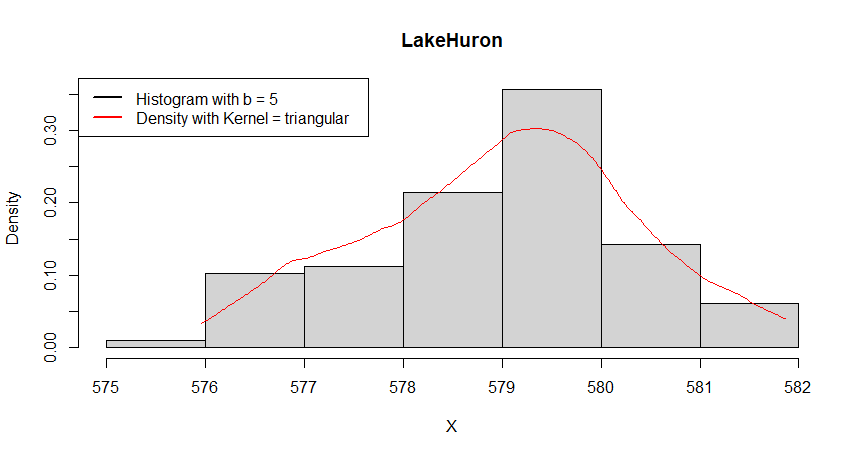
\includegraphics[scale=0.6]{T2_1.png}
\end{problem}


\begin{problem}{5}
\begin{lstlisting}[language=R]
library("pracma")

# sample with gamma distribution
n = 1000
s = rgamma(n, 3, 4)


# x_k
M = 200
x = seq(from=0.01, to=2,length=M)
p <- function(x){
  dgamma(x, 3, 4)
}


legendre_kernel <- function(x){
  (1/2 - 5/8 * (3*x^2 - 1)) * (x < 1) * (x > -1)
}


bandwidth = seq(from=0.1, to=5, by=0.1)
mise_e = vector(len=50)
mise_l = vector(len=50)

for (i in 1:50) {
  D <- density(s, bw=bandwidth[i], kernel=c("epanechnikov"),
	from=0, to=2)
  p_hat <- approx(D$x, D$y, xout=x)
  mise_e[i] <- mean((p(unlist(p_hat[1])) - unlist(p_hat[2]))^2)
  
  p_l = vector(len=200)
  for (j in 1:M) {
    p_l[j] <- mean(
	legendre_kernel((x[j] - s)/bandwidth[i]))/bandwidth[i]  
  }
  mise_l[i] <- mean((p(x) - p_l)^2)
}
plot(mise_e, type="l",col="green")
lines(mise_l, type="l",col="blue")

legend(x = "topright", legend = c("epanechnikov", "legendre"), 
	col = c("green", "blue"), lwd = 2) 


\end{lstlisting}
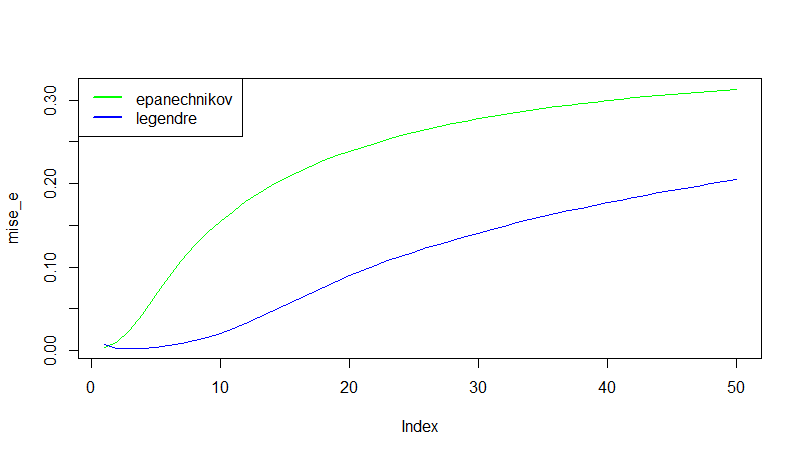
\includegraphics[scale=0.6]{T2_2.png}

\end{problem}
\begin{problem}{5}
\begin{lstlisting}[language=R]
library(mixtools)

N = 1000
eta = sample(1:6, size=N, prob=c(0.5,rep(0.1,5)), replace=TRUE)
m = c(0,seq(from=-1, to=1, by=0.5))
s = c(1,rep(0.1,5))

X = rep(NA, N)
for (k in 1:N){
  X[k]=rnorm(1, mean=m[eta[k]], sd=s[eta[k]])
}

p = function(x){
  y = 0.5 * dnorm(x,0,1)
  for (j in 0:4){
    y = y + 0.1 * dnorm(x, mean=m[j+2], sd=s[j+2])
  }
  return(y)
}

# i
ll = rep(NA, 9)
for (k in 2:10) {
  gm <- normalmixEM(X, k=k, maxit=2500)
  ll[k-1] <- gm$loglik
  print(gm$loglik)
}
which(ll==max(ll))[1]

gm <- normalmixEM(X, k=(which(ll==max(ll))[1]+1), maxit=2500)

p_em <- function(x){
  y = 0
  for (j in 1:(which(ll==max(ll))[1] + 1)){
    y = y + gm$lambda[j] * dnorm(x, mean=gm$mu[j], sd=gm$sigma[j])
  }
  return(y)
}

u=seq(from=-3.5,to=3.5,length=1000)
plot(sapply(u,p_em)~u,type="l",col="red", ylim=c(0,max(sapply(u,p_em))))
lines(sapply(u,p)~u,type="l",col="green")

legend(x = "topright", legend = c("Bart Simpson (EM)",
"Bart Simpson (actual))"), col = c("red", "green"), lwd = 2) 

# ii
D_ucv <- density(X, bw = "ucv", from=-3, to=3 )
D_bcv <- density(X, bw = "bcv", from=-3, to=3 )
plot(unlist(D_ucv[1]), unlist(D_ucv[2]),type="l",col="blue")
lines(unlist(D_bcv[1]), unlist(D_bcv[2]),type="l",col="red")
lines(sapply(u,p)~u,type="l",col="green")

legend(x = "topleft", legend = 
         c("Bart Simpson (kernel ucv)",
           "Bart Simpson (kernel bcv)",
           "Bart Simpson (actual)"), col = c("blue", "red", "green"),
       lwd = 2) 

mean((p_em(unlist(D_ucv$x)) - D_ucv$y)^2)
mean((p_em(unlist(D_bcv$x)) - D_bcv$y)^2)

\end{lstlisting}
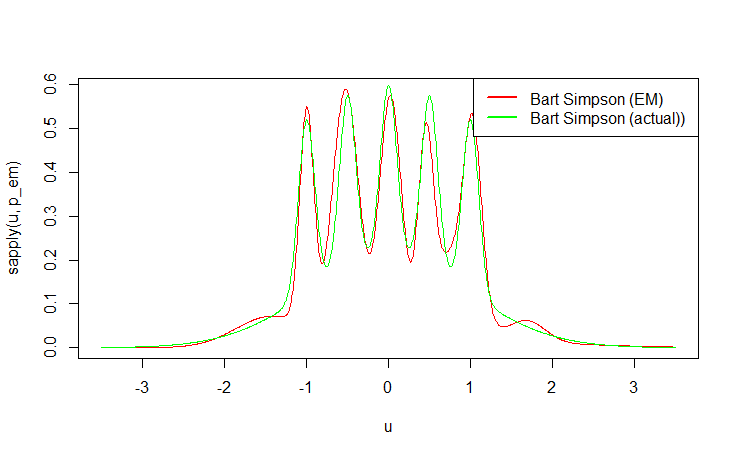
\includegraphics[scale=0.6]{T2_31.png}

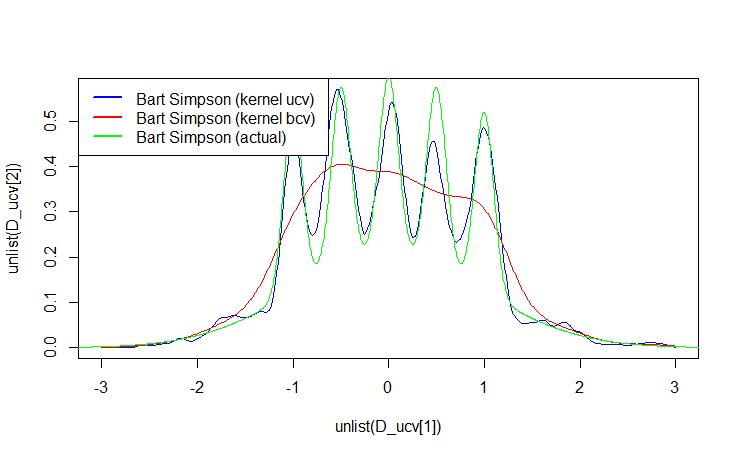
\includegraphics[scale=0.6]{T2_32.png}

\end{problem}
\end{document}
  